
\section{等离子体物理}
\subsection{经典理论}

\subsubsection{本征波动}
记\(\alpha\)类型粒子的质量为\(m_\alpha\)、电荷量为\(q_\alpha\)、未扰动时数密度为\(n_{\alpha 0}\)、声速为\(c_\alpha\)（即分压为\(P_\alpha = m_\alpha c_\alpha^2 n_\alpha\)），体系存在匀强外磁场\(B_0 \uv{b}\).

体系演化方程为
\begin{equation*}
	&n_\alpha m_\alpha \left( \frac{\partial \vb{u}_\alpha}{\partial t} + \vb{u}_\alpha\cdot\nabla \vb{u}_\alpha \right) = -\nabla P_\alpha + n_\alpha q_\alpha \left( \vb{E} + \vb{u}_\alpha\times\vb{B} \right). \\
	&\frac{\partial n_\alpha}{\partial t} + \nabla\cdot\left(n_\alpha \vb{u}_\alpha\right) = 0,\quad \nabla\cdot\vb{E} = \frac{1}{\varepsilon_0}\sum_\beta n_\beta q_\beta.
\end{equation*}

假设未扰动时体系电中性
\begin{equation*}
	\sum_\alpha n_{\alpha 0} q_\alpha = 0,\quad\vb{E} = 0
\end{equation*}

扰动后记
\begin{equation*}
	n_\alpha = n_{\alpha 0} + n_{\alpha 1},\quad
	\vb{E} = -\nabla\phi,\quad
	\Omega_\alpha = \frac{q_\alpha B_0}{m_\alpha},\quad
	\omega_{p\alpha} = \sqrt{\frac{q_\alpha^2 n_{\alpha 0}}{\varepsilon_0 m_\alpha}}.
\end{equation*}

保留至方程线性项，得
\begin{equation*}
	&\nabla^2\phi = -\frac{1}{\varepsilon_0}\sum_\beta n_{\beta 1} q_\beta,\quad
	\frac{\partial n_{\alpha 1}}{\partial t} + n_{\alpha 0}\nabla\cdot\vb{u}_\alpha = 0. \\
	&\frac{\partial \vb{u}_\alpha}{\partial t} = -\frac{c_\alpha^2}{n_{\alpha 0}}\nabla n_{\alpha 1} - \frac{q_\alpha}{m_\alpha}\nabla\phi - \Omega_\alpha \uv{b}\times\vb{u}_\alpha.
\end{equation*}

取波动解，时谐因子记为\(e^{i\left( \vb{k}\cdot\vb{r} - \omega t \right)}\)，得
\begin{equation*}
	&n_{\alpha 1} = n_{\alpha 0}\frac{\vb{k}}{\omega}\cdot\vb{u}_\alpha,\quad
	\phi = \frac{1}{\omega k \varepsilon_0}\uv{k}\cdot\vb{J},\quad\vb{J} = \sum_\alpha n_{\alpha 0} q_\alpha \vb{u}_\alpha,\\
	&\left( \vb{I} - i\frac{\Omega_\alpha}{\omega}\uv{b}\cdot\vb{\epsilon} - \frac{k^2 c_\alpha^2}{\omega^2}\uv{k}\uv{k} \right)\cdot\vb{u}_\alpha + \frac{\omega_{p\alpha}^2}{\omega^2 n_{\alpha 0} q_\alpha}\uv{k}\uv{k}\cdot\vb{J} = 0.
\end{equation*}
其中\(\vb{\epsilon}\)是Levi-Civita张量，若\(\uv{b} = \uv{e}_3\)，\(\uv{e}_1-\uv{e}_2-\uv{e}_3\)构成右手系，则\(\uv{b}\cdot\vb{\epsilon} = \uv{e}_1\uv{e}_2 - \uv{e}_2\uv{e}_1.\)

进而给出本征方程
\begin{equation*}
	\left( \vb{I} - \sum_\alpha \frac{\omega_{p\alpha}^2}{\omega^2}\left( \vb{I} - i\frac{\Omega_\alpha}{\omega}\uv{b}\cdot\vb{\epsilon} - \frac{k^2 c_\alpha^2}{\omega^2}\uv{k}\uv{k} \right)^{-1}\cdot\uv{k}\uv{k} \right)\cdot\vb{J} = 0.
\end{equation*}

记
\begin{equation*}
	&a_\alpha = \frac{\Omega_\alpha}{\omega},\quad
	\beta_\alpha = \frac{k^2 c_\alpha^2}{\omega^2},\quad
	\Delta_\alpha = 1 - a_\alpha^2 - \beta_\alpha\left(1 - a_\alpha^2 \left( \uv{b}\cdot\uv{k} \right)^2\right)\\
	&\uv{e}_1 = \frac{\uv{b}\times\uv{k}}{\left| \uv{b}\times\uv{k} \right|},\quad
	\uv{e}_2 = \frac{\uv{b} - \left( \uv{b}\cdot\uv{k} \right)\uv{k}}{\left| \uv{b}\times\uv{k} \right|},\quad
	\uv{e}_3 = \uv{k}.
\end{equation*}

则逆矩阵可以写作
\begin{equation*}
	& \left( \vb{I} - i a_\alpha \uv{b}\cdot\vb{\epsilon} - \beta_\alpha \uv{k} \uv{k} \right)^{-1} = \frac{1}{\Delta_\alpha}\bigg( (1-\beta_\alpha)\uv{e}_1\uv{e}_1 + \left(1-\beta_\alpha - a_\alpha^2 \left| \uv{b}\times\uv{k} \right|^2\right)\uv{e}_2\uv{e}_2 + \left(1 - a_\alpha^2 \left( \uv{b}\cdot\uv{k} \right)^2\right)\uv{e}_3\uv{e}_3 \bigg. \\
	& \qquad\quad- i a_\alpha \left| \uv{b}\times\uv{k} \right|\left( \uv{e}_1\uv{e}_3 - \uv{e}_3\uv{e}_1 \right) - i a_\alpha \left( \uv{b}\cdot\uv{k} \right)(1-\beta_\alpha)\left( \uv{e}_2\uv{e}_1 - \uv{e}_1\uv{e}_2 \right)- a_\alpha^2\left( \uv{b}\cdot\uv{k} \right) \left| \uv{b}\times\uv{k} \right|\left( \uv{e}_2\uv{e}_3 + \uv{e}_3\uv{e}_2 \right) \bigg).
\end{equation*}

最终代入\(\uv{e}_1, \uv{e}_2, \uv{e}_3\)，可以将本征方程化简为
\begin{equation*}
	\left( \vb{I} - \sum_\alpha \frac{\omega_{p\alpha}^2}{\omega^2}\cdot\frac{\uv{k}\uv{k} - a_\alpha^2\left( \uv{b}\cdot\uv{k} \right)\uv{b}\uv{k} - i a_\alpha\left( \uv{b}\times\uv{k} \right)\uv{k}}{1 - a_\alpha^2 - \beta_\alpha\left(1 - a_\alpha^2\left( \uv{b}\cdot\uv{k} \right)^2\right)} \right)\cdot\vb{J} = 0.
\end{equation*}

记\(\uv{k}\)和\(\uv{b}\)夹角为\(\theta\)，由行列式为零得到色散方程
\begin{equation*}
	\sum_\alpha \frac{\omega_{p\alpha}^2\left(1 - a_\alpha^2\left( \uv{b}\cdot\uv{k} \right)^2\right)}{\omega^2\left(1 - a_\alpha^2 - \beta_\alpha\left(1 - a_\alpha^2\left( \uv{b}\cdot\uv{k} \right)^2\right)\right)}=
	\sum_\alpha \dfrac{\omega_{p\alpha}^2\left(1 + \dfrac{\Omega_\alpha^2\sin^2\theta}{\omega^2 - \Omega_\alpha^2}\right)}{\omega^2 - k^2 c_\alpha^2\left(1 + \dfrac{\Omega_\alpha^2\sin^2\theta}{\omega^2 - \Omega_\alpha^2}\right)} = 1.
\end{equation*}

可见，平行于磁场传播\((\theta = 0)\)等价于不存在磁场\((\Omega_\alpha = 0)\)，均满足色散关系
\begin{equation*}
	\sum_\alpha \frac{\omega_{p\alpha}^2}{\omega^2 - k^2 c_\alpha^2} = 1.
\end{equation*}

垂直于磁场传播\((\theta = \pi/2)\)的色散关系则为
\begin{equation*}
	\sum_\alpha \frac{\omega_{p\alpha}^2}{\omega^2 - k^2 c_\alpha^2 - \Omega_\alpha^2} = 1.
\end{equation*}

最简单的，当等离子体由两类粒子组成，则色散方程给出
\begin{equation*}
	&\left( \omega^2 - \left(k^2 c_1^2 + \omega_{p1}^2\right)\left(1 + \frac{\Omega_1^2\sin^2\theta}{\omega^2 - \Omega_1^2}\right) \right)\cdot\left( \omega^2 - \left(k^2 c_2^2 + \omega_{p2}^2\right)\left(1 + \frac{\Omega_2^2\sin^2\theta}{\omega^2 - \Omega_2^2}\right) \right)\\&\qquad- \omega_{p1}^2 \omega_{p2}^2 \left(1 + \frac{\Omega_1^2\sin^2\theta}{\omega^2 - \Omega_1^2}\right)\left(1 + \frac{\Omega_2^2\sin^2\theta}{\omega^2 - \Omega_2^2}\right) = 0.
\end{equation*}

\subsubsection{电磁响应}
再来考虑该等离子体对外电场的响应，此时 \(\vb{E}\propto e^{-i\omega t}\)，而等离子体内部的数密度波动效应可忽略.线性化的动量方程给出
\begin{equation*}
	m_\alpha \frac{\partial \vb{u}_\alpha}{\partial t} = q_\alpha \left( \vb{E} + \vb{u}_\alpha\times B_0\, \uv{b} \right).
\end{equation*}
受迫解为

\begin{equation*}
	\vb{u}_\alpha &= \frac{i\omega q_\alpha}{m_\alpha \left( \omega^2 - \Omega_\alpha^2 \right)} \left( \vb{I} - \frac{\Omega_\alpha^2}{\omega^2}\uv{b}\uv{b} + i\frac{\Omega_\alpha}{\omega}\uv{b}\cdot\vb{\epsilon} \right)\cdot\vb{E}\\
	\vb{J} &= \sum_\alpha n_{\alpha 0} q_\alpha \vb{u}_\alpha = i\omega\varepsilon_0 \sum_\alpha \frac{\omega_{p\alpha}^2}{\omega^2 - \Omega_\alpha^2}\left( \vb{I} - \frac{\Omega_\alpha^2}{\omega^2}\uv{b}\uv{b} + i\frac{\Omega_\alpha}{\omega}\uv{b}\cdot\vb{\epsilon} \right)\cdot\vb{E}= \vb{\sigma}\cdot\vb{E}.
\end{equation*}
其中 \(\vb{\sigma}\) 为电导率张量，进而相对介电常数张量为
\begin{equation*}
	\vb{\varepsilon}_r = \vb{I} + \frac{i\vb{\sigma}}{\omega\varepsilon_0} = \left(1 - \sum_\alpha \frac{\omega_{p\alpha}^2}{\omega^2 - \Omega_\alpha^2}\right)\vb{I} + \sum_\alpha \frac{\omega_{p\alpha}^2 \Omega_\alpha^2}{\omega^2\left( \omega^2 - \Omega_\alpha^2 \right)}\uv{b}\uv{b} - \sum_\alpha \frac{i\omega_{p\alpha}^2 \Omega_\alpha}{\omega\left( \omega^2 - \Omega_\alpha^2 \right)}\uv{b}\cdot\vb{\epsilon}.
\end{equation*}

由波动方程
\begin{equation*}
	\vb{k}\times\left( \vb{k}\times\vb{E} \right) + \frac{\omega^2}{c^2}\vb{\varepsilon}_r\cdot\vb{E} = 0.
\end{equation*}
记 \(n = kc/\omega\)，得到本征方程为
\begin{equation*}
	\left( \left(1 - n^2 - \sum_\alpha \frac{\omega_{p\alpha}^2}{\omega^2 - \Omega_\alpha^2}\right)\vb{I} + \sum_\alpha \frac{\omega_{p\alpha}^2 \Omega_\alpha^2}{\omega^2\left( \omega^2 - \Omega_\alpha^2 \right)}\uv{b}\uv{b} - \sum_\alpha \frac{i\omega_{p\alpha}^2 \Omega_\alpha}{\omega\left( \omega^2 - \Omega_\alpha^2 \right)}\uv{b}\cdot\vb{\epsilon} + n^2\uv{k}\uv{k} \right)\cdot\vb{E} = 0.
\end{equation*}

记 \(\uv{k}\) 与 \(\uv{b}\) 夹角为 \(\theta\)，行列式为零得到
\begin{equation*}
	&\tan^2\theta = \frac{2n_p^2\left(n^2 - n_R^2\right)\left(n^2 - n_L^2\right)}{\left( \left(n_R^2 + n_L^2\right)n^2 - 2n_R^2 n_L^2 \right)\left(n_p^2 - n^2\right)}\\
	&n_p^2 = 1 - \sum_\alpha \frac{\omega_{p\alpha}^2}{\omega^2},\quad
	n_R^2 = 1 - \sum_\alpha \frac{\omega_{p\alpha}^2}{\omega\left( \omega + \Omega_\alpha \right)},\quad
	n_L^2 = 1 - \sum_\alpha \frac{\omega_{p\alpha}^2}{\omega\left( \omega - \Omega_\alpha \right)}.
\end{equation*}

一般情况下，\(n^2(\theta)\) 是二次方程，将给出两种模式.不难看出，沿磁场方向传播 \((\theta = 0)\) 时，给出左旋 \((n = n_L)\)、右旋 \((n = n_R)\) 圆偏振两种模式.垂直于磁场传播 \((\theta = \pi/2)\) 时，给出两种模式
\begin{equation*}
	n &= n_p,\quad \vb{E}\cdot\uv{b}\neq0,\quad \vb{E}\times\uv{b} = 0. \\
	n &= \sqrt{\frac{2n_R^2 n_L^2}{n_R^2 + n_L^2}},\quad \vb{E}\cdot\uv{b} = 0,\quad \frac{\vb{E}\cdot\uv{k}}{\vb{E}\cdot\left( \uv{b}\times\uv{k} \right)} = \frac{i\left(n_R^2 - n_L^2\right)}{n_R^2 + n_L^2}.
\end{equation*}

\subsection{动理学理论}

\subsubsection{外磁场下的电磁响应}
记\(\alpha\)类型粒子的质量为\(m_\alpha\)、电荷量为\(q_\alpha\)、数密度为\(n_\alpha\)、温度为\(T_\alpha\)，特征角频率\(\omega_{p\alpha}\)、热速率\(v_{\text{th}\alpha}\)、屏蔽长度\(\lambda_{D\alpha}\)为（后两者暂时用不到）
\begin{equation*}
	\omega_{p\alpha} = \sqrt{\frac{n_\alpha q_\alpha^2}{\varepsilon_0 m_\alpha}},\quad
	v_{\text{th}\alpha} = \sqrt{\frac{2k_B T_\alpha}{m_\alpha}},\quad
	\lambda_{D\alpha} = \sqrt{\frac{\varepsilon_0 k_B T_\alpha}{n_\alpha q_\alpha^2}}.
\end{equation*}

相空间分布函数 \(f_\alpha\left( \vb{r},\vb{v},t \right)\) 满足归一化条件
\begin{equation*}
	\iint f_\alpha\left( \vb{r},\vb{v},t \right)\d \vb{r}\d \vb{v} = 1.
\end{equation*}

在电磁场的作用下，从最原始的碰撞方程出发
\begin{equation*}
	\frac{\d f_\alpha}{\d t} = \frac{\partial f_\alpha}{\partial t} + \vb{v}\cdot\frac{\partial f_\alpha}{\partial \vb{r}} + \frac{q_\alpha}{m_\alpha}\left( \vb{E} + \vb{v}\times\vb{B} \right)\cdot\frac{\partial f_\alpha}{\partial \vb{v}} = 0.
\end{equation*}

假设未扰动时，分布是均匀的，分布函数可以分为
\begin{equation*}
	f_\alpha\left( \vb{r},\vb{v},t \right) = f_{\alpha0}\left( \vb{v} \right) + \delta f_\alpha\left( \vb{r},\vb{v},t \right)
\end{equation*}
其中 \(f_{\alpha0}\left( \vb{v} \right)\) 正比于粒子数密度 \(n_\alpha\).

先考虑空间存在匀强外磁场 \(\vb{B}_0\) 的情形，则
\begin{equation*}
	&\frac{q_\alpha B_0}{m_\alpha}\vb{v}\times\uv{b}\cdot\frac{\partial f_{\alpha0}}{\partial \vb{v}} = -\vb{v}\cdot\frac{\partial f_{\alpha0}}{\partial \vb{r}}. \\
	&\frac{\d \delta f_\alpha}{\d t} = \frac{\partial \delta f_\alpha}{\partial t} + \vb{v}\cdot\frac{\partial \delta f_{\alpha0}}{\partial \vb{r}} = -\frac{q_\alpha}{m_\alpha}\left( \delta\vb{E} + \vb{v}\times\delta\vb{B} \right)\cdot\frac{\partial f_{\alpha0}}{\partial \vb{v}}.
\end{equation*}
\begin{figure}[htbp]
	\centering
	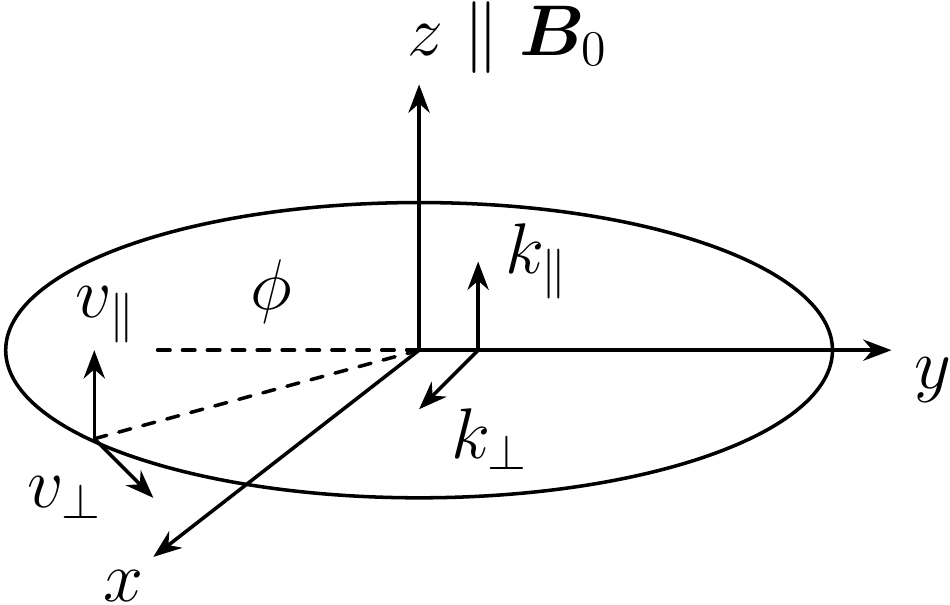
\includegraphics[width=0.35\textwidth]{plasma_fig/cyclotron_motion_schematic_diagram.png}
	\caption{回旋运动示意图}
	\label{回旋运动示意图}
\end{figure}

前一个方程中，记
\begin{equation*}
	\vb{B}_0 = B_0 \uv{z}, \quad
	\Omega_\alpha = \frac{q_\alpha B_0}{m_\alpha}.
\end{equation*}
如图\ref{回旋运动示意图}，粒子做回旋运动，速度可写作
\begin{equation*}
	\vb{v} = v_\perp\left( \cos\phi\,\uv{x} + \sin\phi\,\uv{y} \right) + v_\parallel \,\uv{z}.
\end{equation*}
由于粒子是均匀的，因此
\begin{equation*}
	\vb{v}\times\uv{b}\cdot\frac{\partial f_{\alpha0}}{\partial \vb{v}} = -\frac{\partial f_{\alpha0}}{\partial \phi} = 0 \implies f_{\alpha0}\left( \vb{v} \right) = f_{\alpha0}\left( v_\parallel, v_\perp \right).
\end{equation*}

后一个方程给出
\begin{equation*}
	\delta f_\alpha\left( \vb{r},\vb{v},t \right) = -\frac{q_\alpha}{m_\alpha}\int_{-\infty}^t \d t'\left( \delta\vb{E}\left( \vb{r}',t' \right) + \vb{v}'(t')\times\delta\vb{B}\left( \vb{r}',t' \right) \right)\cdot\frac{\partial f_{\alpha0}\left( \vb{v}' \right)}{\partial \vb{v}'}.
\end{equation*}
这里 \(\vb{v}'(t')\) 可以根据匀强磁场中的回旋运动求得，记 \(\tau = t-t'\)，则
\begin{equation*}
	\frac{\d^2 \vb{r}'}{\d \tau^2} = -\frac{\d \vb{v}'}{\d \tau} = \Omega_\alpha \uv{z}\times\vb{v}',\quad
	\left.\vb{r}'\right|_{\tau=0} = \vb{r},\ \left.\vb{v}'\right|_{\tau=0} = \vb{v}.
\end{equation*}
解得
\begin{equation*}
	&\vb{v}' = v_\parallel \uv{z} + v_\perp\left( \cos\left( \Omega_\alpha\tau+\phi \right)\uv{x} + \sin\left( \Omega_\alpha\tau+\phi \right)\uv{y} \right). \\
	&\vb{r}' - \vb{r} = -v_\parallel \tau \uv{z} - \frac{v_\perp}{\Omega_\alpha}\left( \sin\left( \Omega_\alpha\tau+\phi \right)-\sin\phi \right)\uv{x} + \frac{v_\perp}{\Omega_\alpha}\left( \cos\left( \Omega_\alpha\tau+\phi \right)-\cos\phi \right)\uv{y},\\
	&\frac{\partial f_{\alpha0}}{\partial \vb{v}'} = \frac{\partial f_{\alpha0}}{\partial v_\perp}\left( \cos\left( \Omega_\alpha\tau+\phi \right)\uv{x} + \sin\left( \Omega_\alpha\tau+\phi \right)\uv{y} \right) + \frac{\partial f_{\alpha0}}{\partial v_\parallel}\uv{z}.
\end{equation*}

回代上式，同时对分布函数和电磁场的时间空间变量同时做傅里叶变换
\begin{equation*}
	&\mathcal{F}_\alpha\left( \vb{k},\vb{v},\omega \right) = \frac{1}{\left(2\pi\right)^2}\iint \delta f_\alpha\left( \vb{r},\vb{v},t \right)e^{-i\left( \vb{k}\cdot\vb{r}-\omega t \right)}\,\d \vb{r}\,\d t,\\
	&\delta\vb{E}\left( \vb{r},t \right) \to \mathcal{E}\left( \vb{k},\omega \right),\quad
	\delta\vb{B}\left( \vb{r},t \right) \to \mathcal{B}\left( \vb{k},\omega \right),\quad\nabla \times \vb{E} = -\frac{\partial \vb{B}}{\partial t} \to \mathcal{B}\left( \vb{k},\omega \right) = \frac{\vb{k}}{\omega} \times \mathcal{E}\left( \vb{k},\omega \right).
\end{equation*}
得到分布函数扰动量为
\begin{equation*}
	\mathcal{F}_\alpha &= -\frac{q_\alpha}{m_\alpha}\int_0^\infty\!\!\left( \mathcal{E}+\frac{\vb{v}'\times\left( \vb{k}\times\mathcal{E} \right)}{\omega} \right)\!\cdot\frac{\partial f_{\alpha0}}{\partial \vb{v}'} e^{i\left( \vb{k}\cdot\left( \vb{r}'-\vb{r} \right)+\omega\tau \right)}\d \tau \\&= -\frac{q_\alpha}{m_\alpha}\sum_{m,n=-\infty}^{\infty}\int_0^\infty\!\!\Bigg\{ \Bigg( \frac{\partial f_{\alpha0}}{\partial v_\perp}+\frac{k_\parallel v_\perp}{\omega}\frac{\partial f_{\alpha0}}{\partial v_\parallel}-\frac{k_\parallel v_\parallel}{\omega}\frac{\partial f_{\alpha0}}{\partial v_\perp} \Bigg)\left( \cos\left(\Omega_\alpha\tau+\phi\right)\mathcal{E}_x+\sin\left(\Omega_\alpha\tau+\phi\right)\mathcal{E}_y \right) \\&\quad\quad+ \Bigg( \frac{\partial f_{\alpha0}}{\partial v_\parallel}-\frac{k_\perp}{\omega}\left( v_\perp\frac{\partial f_{\alpha0}}{\partial v_\parallel}-v_\parallel\frac{\partial f_{\alpha0}}{\partial v_\perp} \right)\cos(\Omega_\alpha\tau+\phi) \Bigg)\mathcal{E}_z \Bigg\}J_m(\xi_\alpha)J_n(\xi_\alpha)e^{i\left( \omega-n\Omega_\alpha-k_\parallel v_\parallel \right)\tau}e^{i(m-n)\phi}\d \tau.
\end{equation*}
其中贝塞尔函数宗量为 \(\xi_\alpha = k_\perp v_\perp/\Omega_\alpha\)，选取 \(x\) 轴使得 \(\vb{k} = k_\parallel \uv{z} + k_\perp \uv{x}\).

体系原先电中性，故扰动后电流密度为
\begin{equation*}
	\vb{J}\left( \vb{r},t \right) = \sum_\alpha \int q_\alpha \vb{v}\,\delta f_\alpha\left( \vb{r},\vb{v},t \right)\d \vb{v}.
\end{equation*}

做傅里叶变换后，电流密度显然可以写成关于电场强度的线性形式
\begin{equation*}
	\mathcal{J}\left( \vb{k},\omega \right) = \sum_\alpha \int q_\alpha \vb{v}\,\mathcal{F}_\alpha\left( \vb{k},\vb{v},\omega \right)\d \vb{v} = \vb{\sigma}(\omega)\cdot\mathcal{E}\left( \vb{k},\omega \right).
\end{equation*}

进而根据电导率张量 \(\vb{\sigma}\)，完成积分，得到介电常量张量为（贝塞尔函数下标\(\alpha\)指宗量为\(\xi_\alpha\)）
\begin{equation*}
	\vb{\varepsilon}_r(\omega) &= \vb{I} + \frac{i\vb{\sigma}(\omega)}{\varepsilon_0 \omega} = \vb{I} + \sum_\alpha \frac{\omega_{p\alpha}^2}{\omega^2 n_\alpha}\sum_{n=-\infty}^{\infty}\int\frac{\vb{S}_{\alpha n}}{\omega-n\Omega_\alpha-k_\parallel v_\parallel}\d \vb{v}\\
	\vb{S}_{\alpha n}&=
	\begin{pmatrix}
		v_\perp\left( \dfrac{nJ_{n\alpha}}{\xi_\alpha} \right)^2 U_\alpha & i v_\perp \dfrac{n}{\xi_\alpha}J_{n\alpha}J_{n\alpha}'U_\alpha & v_\perp \dfrac{n}{\xi_\alpha}J_{n\alpha}^2 W_{\alpha n} \\[8pt]
		-i v_\perp \dfrac{n}{\xi_\alpha}J_{n\alpha}J_{n\alpha}'U_\alpha   & v_\perp \left( J_{n\alpha}' \right)^2 U_\alpha                 & -i v_\perp J_{n\alpha}J_{n\alpha}' W_{\alpha n}         \\[8pt]
		v_\parallel \dfrac{n}{\xi_\alpha}J_{n\alpha}^2 U_\alpha           & i v_\parallel J_{n\alpha}J_{n\alpha}' U_\alpha                 & v_\parallel J_{n\alpha}^2 W_{\alpha n}
	\end{pmatrix}.\\
	U_\alpha &= \left( \omega - k_\parallel v_\parallel \right)\frac{\partial f_{\alpha0}}{\partial v_\perp} + v_\perp k_\parallel \frac{\partial f_{\alpha0}}{\partial v_\parallel}, \quad
	W_{\alpha n} = \frac{n\Omega_\alpha v_\parallel}{v_\perp}\frac{\partial f_{\alpha0}}{\partial v_\perp} + \left( \omega - n\Omega_\alpha \right)\frac{\partial f_{\alpha0}}{\partial v_\parallel}.
\end{equation*}

注意到
\begin{equation*}
	\frac{v_\parallel U_\alpha - v_\perp W_{\alpha}}{\omega - n\Omega_\alpha - k_\parallel v_\parallel} = v_\parallel \frac{\partial f_{\alpha0}}{\partial v_\perp} - v_\perp \frac{\partial f_{\alpha0}}{\partial v_\parallel},\quad
	\sum_{n=-\infty}^{\infty}nJ_n^2(x) = 0.
\end{equation*}

进一步计算得到
\begin{equation*}
	\vb{\varepsilon}_r = \vb{I} + \sum_\alpha \frac{\omega_{p\alpha}^2}{\omega^2 n_\alpha}\sum_{n=-\infty}^{\infty}\int\!\!\Bigg[ \!\left(v_\parallel\frac{\partial f_{\alpha0}}{\partial v_\parallel}-\frac{v_\parallel^2}{v_\perp}\frac{\partial f_{\alpha0}}{\partial v_\perp} \right)\uv{b}\uv{b} + \frac{v_\perp U_\alpha}{\omega-n\Omega_\alpha-k_\parallel v_\parallel}
		\begin{pmatrix}
			\left( \dfrac{nJ_{n\alpha}}{\xi_\alpha} \right)^2              & \dfrac{in}{\xi_\alpha}J_{n\alpha}J_{n\alpha}'        & \dfrac{v_\parallel}{v_\perp}\dfrac{n}{\xi_\alpha}J_{n\alpha}^2 \\[8pt]
			\dfrac{n}{i\xi_\alpha}J_{n\alpha}J_{n\alpha}'                  & \left( J_{n\alpha}' \right)^2                        & \dfrac{v_\parallel}{iv_\perp}J_{n\alpha}J_{n\alpha}'           \\[8pt]
			\dfrac{v_\parallel}{v_\perp}\dfrac{n}{\xi_\alpha}J_{n\alpha}^2 & \dfrac{iv_\parallel}{v_\perp}J_{n\alpha}J_{n\alpha}' & \dfrac{v_\parallel^2}{v_\perp^2}J_{n\alpha}^2
		\end{pmatrix}\Bigg]\d \vb{v}.
\end{equation*}

不难看到，\(\vb{\varepsilon}_r\) 满足线性系统一般的Onsager关系
\begin{equation*}
	\vb{\varepsilon}_r\left( \vb{B}_0 \right) = \vb{\varepsilon}_r^\mathrm{T}\left( -\vb{B}_0 \right).
\end{equation*}

之后，将介电常量张量代入波动方程
\begin{equation*}
	\vb{k}\times\left( \vb{k}\times\mathcal{E} \right) + \frac{\omega^2}{c^2}\vb{\varepsilon}_r\cdot\mathcal{E} = \left( \begin{pmatrix} -k_\parallel^2 & 0 & k_\parallel k_\perp \\ 0 & -k^2 & 0 \\ k_\perp & 0 & -k_\perp^2 \end{pmatrix} + \frac{\omega^2}{c^2}\vb{\varepsilon}_r \right)\cdot\mathcal{E} = 0.
\end{equation*}
便可以解出色散关系和偏振模式.

在冷等离子体极限下，特征速率与 \(\Omega_\alpha/k\) 及 \(\omega/k\) 相比为小量，且 \(\xi_\alpha \to 0\)，仅 \(n = 0,\pm1\) 项有贡献，取极限得
\begin{equation*}
	\vb{\varepsilon}_r(\omega) &= \vb{I} + \sum_\alpha\frac{\omega_{p\alpha}^2}{\omega^2 - \Omega_\alpha^2}\left( \vb{I} + i\frac{\Omega_\alpha}{\omega}\uv{b}\cdot\vb{\epsilon} - \uv{b}\uv{b} \right)
	\int\frac{v_\perp}{2n_\alpha}\frac{\partial f_{\alpha0}}{\partial v_\perp}\d \vb{v} + \sum_\alpha\frac{\omega_{p\alpha}^2}{\omega^2}\uv{b}\uv{b}\int\frac{v_{\parallel}}{n_\alpha}\frac{\partial f_{\alpha0}}{\partial v_{\parallel}}\d \vb{v}\\
	&= \left(1 - \sum_\alpha\frac{\omega_{p\alpha}^2}{\omega^2 - \Omega_\alpha^2}\right)\vb{I} + \sum_\alpha\frac{\omega_{p\alpha}^2\Omega_\alpha^2}{\omega^2\left(\omega^2 - \Omega_\alpha^2\right)}\uv{b}\uv{b} - \sum_\alpha\frac{i\omega_{p\alpha}^2\Omega_\alpha}{\omega\left(\omega^2 - \Omega_\alpha^2\right)}\uv{b}\cdot\vb{\epsilon}.
\end{equation*}
计算中用到
\begin{equation*}
	\int\frac{v_\perp}{2n_\alpha}\frac{\partial f_{\alpha0}}{\partial v_\perp}\d \vb{v} = \int\frac{v_{\parallel}}{n_\alpha}\frac{\partial f_{\alpha0}}{\partial v_{\parallel}}\d \vb{v} = -1,
	\quad
	\uv{b}\uv{b} = \begin{pmatrix}0&0&0\\0&0&0\\0&0&1\end{pmatrix},
	\quad
	\uv{b}\cdot\vb{\epsilon} = \begin{pmatrix}0&1&0\\-1&0&0\\0&0&0\end{pmatrix}.
\end{equation*}
这与前面的结果完全一致.

在一般情形下，若不给定 \(f_{\alpha0}\)，以上方程已无法再化简，直观起见，假设未扰动时，粒子满足各向同性的Maxwell速率分布
\begin{equation*}
	f_{\alpha0}\left(v_{\parallel},v_\perp\right) = \frac{n_\alpha}{\pi^{3/2}v_{\mathrm{th}\alpha}^3}\mathrm{e}^{-\frac{v_{\parallel}^2 + v_\perp^2}{v_{\mathrm{th}\alpha}^2}}.
\end{equation*}
则介电常量张量可化简为
\begin{equation*}
	\vb{\varepsilon}_r(\omega) = \vb{I} + \sum_\alpha\frac{\omega_{p\alpha}^2\mathrm{e}^{-\kappa_\alpha}}{\omega k_{\parallel}v_{\mathrm{th}\alpha}}
	\sum_{n=-\infty}^{\infty}
	\begin{pmatrix}
		\dfrac{n^2I_{n\alpha}Z_\alpha}{\kappa_\alpha}               & in\left(I_{n\alpha}-I_{n\alpha}^\prime\right)Z_\alpha                                                                & -nI_{n\alpha}Z_\alpha^\prime\sqrt{\dfrac{2}{\kappa_\alpha}}                       \\[6pt]
		in\left(I_{n\alpha}-I_{n\alpha}^\prime\right)Z_\alpha       & \left(\dfrac{n^2I_{n\alpha}}{\kappa_\alpha}+2\kappa_\alpha\left(I_{n\alpha}-I_{n\alpha}^\prime\right)\right)Z_\alpha & -i\sqrt{2\kappa_\alpha}\left(I_{n\alpha}-I_{n\alpha}^\prime\right)Z_\alpha^\prime \\[6pt]
		-nI_{n\alpha}Z_\alpha^\prime\sqrt{\dfrac{2}{\kappa_\alpha}} & i\sqrt{2\kappa_\alpha}\left(I_{n\alpha}-I_{n\alpha}^\prime\right)Z_\alpha^\prime                                     & -\chi_{\alpha,n}I_{n\alpha}Z_\alpha^\prime
	\end{pmatrix}
\end{equation*}
其中修正贝塞尔函数下标\(\alpha\)指宗量为 \(\kappa_\alpha\)，等离子体色散函数 \(Z(\zeta)\) 下标\(\alpha\)指宗量为 \(\chi_{\alpha,n}\)
\begin{equation*}
	\kappa_\alpha = \frac{k_\perp^2v_{\mathrm{th}\alpha}^2}{2\Omega_\alpha^2}, \quad \chi_{\alpha,n} = \frac{\omega - n\Omega_\alpha}{k_{\parallel}v_{\mathrm{th}\alpha}}.
\end{equation*}
计算中用到数学公式 (\(Z(\zeta)\) 称为等离子体色散函数)
\begin{equation*}
	\mathrm{e}^{\kappa}\int_{0}^{\infty}t\mathrm{e}^{-t^2}J_n^2\left(t\sqrt{2\kappa}\right)\d t = \frac{1}{2}I_n(\kappa).
\end{equation*}
\begin{equation*}
	Z(\zeta) = \frac{1}{\sqrt{\pi}}\int_{-\infty}^{\infty}\frac{\mathrm{e}^{-u^2}}{u-\zeta}\d u, \quad Z'(\zeta) = -2\left(1+\zeta Z(\zeta)\right) = -\frac{2}{\sqrt{\pi}}\int_{-\infty}^{\infty}\frac{u\mathrm{e}^{-u^2}}{u-\zeta}\d u.
\end{equation*}

\begin{example}
	波矢平行于外磁场

	此时\(k_\perp=0, k_{\parallel}=k\)，此时仅 \(n=\pm1\) 项有贡献 \(\left(I_{\pm1}(\kappa_\alpha)=\kappa_\alpha/2+\mathcal{O}(\kappa_\alpha^3)\right)\)，化简得
	\begin{equation*}
		\vb{\varepsilon}_r(\omega) = \vb{I} + \sum_\alpha\frac{\omega_{p\alpha}^2}{2\omega k v_{\mathrm{th}\alpha}}
		\begin{pmatrix}
			Z(\chi_{\alpha,1})+Z(\chi_{\alpha,-1})                & i\left(Z(\chi_{\alpha,1})-Z(\chi_{\alpha,-1})\right) & 0                                    \\
			-i\left(Z(\chi_{\alpha,1})-Z(\chi_{\alpha,-1})\right) & Z(\chi_{\alpha,1})+Z(\chi_{\alpha,-1})               & 0                                    \\
			0                                                     & 0                                                    & -2\chi_{\alpha,0}Z'(\chi_{\alpha,0})
		\end{pmatrix}.
	\end{equation*}
	\begin{equation*}
		\chi_{\alpha,0} = \frac{\omega}{k v_{\mathrm{th}\alpha}},\quad \chi_{\alpha,\pm1} = \frac{\omega\mp\Omega_{c\alpha}}{k v_{\mathrm{th}\alpha}}.
	\end{equation*}
	回代波动方程，得到色散关系
	\begin{equation*}
		1 + 2\sum_\alpha\frac{\omega_{p\alpha}^2}{\left(k v_{\mathrm{th}\alpha}\right)^2}\left(1+\frac{\omega}{k v_{\mathrm{th}\alpha}}Z\left(\frac{\omega}{k v_{\mathrm{th}\alpha}}\right)\right) = 0.
	\end{equation*}
	或
	\begin{equation*}
		1 - \frac{k^2c^2}{\omega^2} + \sum_\alpha\frac{\omega_{p\alpha}^2}{\omega k v_{\mathrm{th}\alpha}}Z\left(\frac{\omega\mp\Omega_{c\alpha}}{k v_{\mathrm{th}\alpha}}\right) = 0.
	\end{equation*}
	后两支色散关系恰好对应左/右旋圆偏振模式.
\end{example}

\begin{example}
	波矢垂直于外磁场

	此时\(k_{\parallel}=0, k_\perp=k, \chi_{\alpha,n}\to\infty, Z(\chi_{\alpha,n})\to-\chi_{\alpha,n}^{-1}\)，取极限得
	\begin{equation*}
		\vb{\varepsilon}_r(\omega) = \vb{I} - \sum_\alpha\frac{\omega_{p\alpha}^2\mathrm{e}^{-\kappa_\alpha}}{\omega\kappa_\alpha}
		\sum_{n=-\infty}^{\infty}\frac{1}{\omega-n\Omega_\alpha}
		\begin{pmatrix}
			n^2I_{n\alpha}                                             & -in\kappa_\alpha\left(I_{n\alpha}-I_{n\alpha}^\prime\right)                & 0                         \\
			in\kappa_\alpha\left(I_{n\alpha}-I_{n\alpha}^\prime\right) & n^2I_{n\alpha}+2\kappa_\alpha^2\left(I_{n\alpha}-I_{n\alpha}^\prime\right) & 0                         \\
			0                                                          & 0                                                                          & \kappa_\alpha I_{n\alpha}
		\end{pmatrix}.
	\end{equation*}
	回代波动方程，得到色散关系
	\begin{equation*}
		1 - \frac{k^2c^2}{\omega^2} - \sum_\alpha\frac{\omega_{p\alpha}^2\mathrm{e}^{-\kappa_\alpha}}{\omega}\sum_{n=-\infty}^{\infty}\frac{I_n(\kappa_\alpha)}{\omega-n\Omega_\alpha} = 0.
	\end{equation*}
	或
	\begin{equation*}
		&\Bigg(1 - \sum_\alpha\frac{\omega_{p\alpha}^2\mathrm{e}^{-\kappa_\alpha}}{\omega\kappa_\alpha}\sum_{n=-\infty}^{\infty}\frac{n^2I_n(\kappa_\alpha)}{\omega-n\Omega_\alpha}\Bigg)
		\Bigg(1 - \frac{k^2c^2}{\omega^2} - \sum_\alpha\frac{\omega_{p\alpha}^2\mathrm{e}^{-\kappa_\alpha}}{\omega\kappa_\alpha}\sum_{n=-\infty}^{\infty}\frac{n^2I_n(\kappa_\alpha)+2\kappa_\alpha^2\left(I_n(\kappa_\alpha)-I_n^\prime(\kappa_\alpha)\right)}{\omega-n\Omega_\alpha}\Bigg)\\
		&\qquad= \left[\sum_\alpha\frac{\omega_{p\alpha}^2\mathrm{e}^{-\kappa_\alpha}}{\omega\kappa_\alpha}\sum_{n=-\infty}^{\infty}n\frac{I_n(\kappa_\alpha)-I_n^\prime(\kappa_\alpha)}{\omega-n\Omega_\alpha}\right]^2.
	\end{equation*}
\end{example}

\subsubsection{无外磁场的电磁响应}
需要强调的是，通过对如上介电常量张量取零外磁场极限 \(\left(B_0=0,\Omega_\alpha=0,\xi_\alpha\Omega_\alpha=k_\perp v_\perp\right)\)，并不能得到没有外磁场的普适形式.这是因为 \(B_0\neq0\) 强制要求 \(f_{\alpha0}(\vb{v})=f_{\alpha0}(v_{\parallel},v_\perp)\)，即速度关于 \(\uv{b}\) 的轴对称分布，而 \(B_0=0\) 时不会对 \(f_{\alpha0}(\vb{v})\) 施加任何约束.当然，取极限的数学过程也极其繁琐.

因此对于更为普遍的无磁场情形，应当从头考虑.

无磁场时粒子做匀速运动，故
\begin{equation*}
	\vb{v}^\prime(t^\prime)=\vb{v},\qquad \vb{r}^\prime - \vb{r}=-\vb{v}\tau.
\end{equation*}
代入分布函数扰动，将对\(\tau\)的积分视为拉普拉斯变换，得
\begin{equation*}
	\mathcal{F}_\alpha &= -\frac{q_\alpha}{m_\alpha}\int_{0}^{\infty}\left(\bm{\mathcal{E}}+\frac{\vb{v}^\prime\times\left(\vb{k}\times\bm{\mathcal{E}}\right)}{\omega}\right)\cdot\frac{\partial f_{\alpha0}}{\partial\vb{v}^\prime}\mathrm{e}^{i\left(\vb{k}\cdot\left(\vb{r}^\prime-\vb{r}\right)+\omega\tau\right)}\d \tau\\
	&= -\frac{i}{\omega-\vb{k}\cdot\vb{v}}\frac{q_\alpha}{m_\alpha}\Bigg(\bigg(1-\frac{\vb{k}\cdot\vb{v}}{\omega}\bigg)\frac{\partial f_{\alpha0}}{\partial\vb{v}}+\bigg(\frac{\vb{k}}{\omega}\cdot\frac{\partial f_{\alpha0}}{\partial\vb{v}}\bigg)\vb{v}\Bigg)\cdot\bm{\mathcal{E}}.
\end{equation*}
进而电流密度、电导率张量、介电常量张量可以求得
\begin{equation*}
	&\bm{\mathcal{J}} = \sum_\alpha\int q_\alpha\vb{v}\mathcal{F}_\alpha\d \vb{v} = \vb{\sigma}\cdot\bm{\mathcal{E}},\\
	&\vb{\varepsilon}_r = \vb{I} + \frac{i\vb{\sigma}}{\omega\varepsilon_0} = \vb{I} + \sum_\alpha\int\frac{\omega_{p\alpha}^2}{n_\alpha\omega^2}\bigg(\vb{v}\frac{\partial f_{\alpha0}}{\partial\vb{v}}+\bigg(\frac{\vb{k}}{\omega-\vb{k}\cdot\vb{v}}\cdot\frac{\partial f_{\alpha0}}{\partial\vb{v}}\bigg)\vb{v}\vb{v}\bigg)\d \vb{v}.
\end{equation*}
之后，再代入波动方程
\begin{equation*}
	\vb{k}\times\left(\vb{k}\times\bm{\mathcal{E}}\right) + \frac{\omega^2}{c^2}\vb{\varepsilon}_r\cdot\bm{\mathcal{E}} = 0
\end{equation*}
便可以解出色散关系和偏振模式.

\begin{example}
	当速度分布各向同性
	\begin{equation*}
		\frac{\partial f_{\alpha0}}{\partial\vb{v}} = \frac{\partial f_{\alpha0}}{v \,\partial v}\vb{v}.
	\end{equation*}
	得到介电常量张量为
	\begin{equation*}
		\vb{\varepsilon}_r &= \vb{I} + \sum_\alpha\int\frac{\omega_{p\alpha}^2}{n_\alpha\omega\left(\omega-\vb{k}\cdot\vb{v}\right)}\frac{\partial f_{\alpha0}}{v\,\partial v}\vb{v}\vb{v}\d \vb{v}\\
		&= \vb{I} - \sum_\alpha\int\frac{\omega_{p\alpha}^2f_{\alpha0}}{n_\alpha\omega\left(\omega-\vb{k}\cdot\vb{v}\right)}\d \vb{v}\left(\vb{I}-\uv{k}\uv{k}\right) + \sum_\alpha\int\frac{\omega_{p\alpha}^2\vb{k}\cdot\vb{v}}{n_\alpha k^2\left(\omega-\vb{k}\cdot\vb{v}\right)}\frac{\partial f_{\alpha0}}{v\,\partial v}\d \vb{v}\,\uv{k}\uv{k}.
	\end{equation*}
	可见，其形式与光轴为 \(\uv{k}\) 的单轴晶体相同，相应光学特征便也完全一致.

	代入波动方程，给出色散关系
	\begin{equation*}
		1 - \frac{k^2c^2}{\omega^2} - \sum_\alpha\int\frac{\omega_{p\alpha}^2}{n_\alpha\omega\left(\omega-\vb{k}\cdot\vb{v}\right)}f_{\alpha0}\d \vb{v} = 0.
	\end{equation*}
	或
	\begin{equation*}
		1 + \sum_\alpha\int\frac{\omega_{p\alpha}^2\vb{k}\cdot\vb{v}}{n_\alpha k^2\left(\omega-\vb{k}\cdot\vb{v}\right)}\frac{1}{v}\frac{\partial f_{\alpha0}}{\partial v}\d \vb{v} = 0.
	\end{equation*}
	后者要求电场是纵波 \(\left(\bm{\mathcal{E}}//\uv{k}\right)\)，也是大多数教材中考虑的等离子体色散方程.

	又比如，当速度分布关于波矢方向轴对称时
	\begin{equation*}
		f_{\alpha0}(\vb{v})=f_{\alpha0}(v_{\parallel},v_\perp),\qquad v_{\parallel}=\vb{v}\cdot\uv{k},\qquad v_\perp=|\vb{v}\times\uv{k}|.
	\end{equation*}
	介电常量张量可化简为
	\begin{equation*}
		\vb{\varepsilon}_r = \Bigg(1 + \sum_\alpha\frac{\omega_{p\alpha}^2}{\omega^2}\bigg(-1 + \int\frac{k v_\perp^2}{\omega-k v_{\parallel}}\frac{1}{2n_\alpha}\frac{\partial f_{\alpha0}}{\partial v_{\parallel}}\d \vb{v}\bigg)\Bigg)\left(\vb{I}-\uv{k}\uv{k}\right) + \Bigg(1 + \sum_\alpha\frac{\omega_{p\alpha}^2}{k}\int\frac{1}{\omega-k v_{\parallel}}\frac{1}{n_\alpha}\frac{\partial f_{\alpha0}}{\partial v_{\parallel}}\d \vb{v}\Bigg)\uv{k}\uv{k}.
	\end{equation*}
	形式仍然与光轴为 \(\uv{k}\) 的单轴晶体相同.

	代入波动方程，给出色散关系
	\begin{equation*}
		1 - \frac{k^2c^2}{\omega^2} + \sum_\alpha\frac{\omega_{p\alpha}^2}{\omega^2}\bigg(-1 + \int\frac{k v_\perp^2}{\omega-k v_{\parallel}}\frac{1}{2n_\alpha}\frac{\partial f_{\alpha0}}{\partial v_{\parallel}}\d \vb{v}\bigg) = 0.
	\end{equation*}
	或
	\begin{equation*}
		1 + \sum_\alpha\frac{\omega_{p\alpha}^2}{k}\int\frac{1}{\omega-k v_{\parallel}}\frac{1}{n_\alpha}\frac{\partial f_{\alpha0}}{\partial v_{\parallel}}\d \vb{v} = 0
	\end{equation*}
\end{example}

\begin{example}
	\label{等离子体_横纵可分离变量}

	若速度分布关于横、纵向可分离变量，记
	\begin{equation*}
		F_{\alpha0}(v_{\parallel}) = \int f_{\alpha0}(v_\perp,v_{\parallel})2\pi v_\perp\d v_\perp.
	\end{equation*}
	则
	\begin{equation*}
		\vb{\varepsilon}_r = \vb{I} - \sum_\alpha\frac{\omega_{p\alpha}^2}{\omega^2}\left(\vb{I}-\uv{k}\uv{k}\right) + \sum_\alpha\frac{\omega_{p\alpha}^2}{k}\bigg(\frac{k^2v_{\mathrm{th}\perp\alpha}^2}{2\omega^2}\left(\vb{I}-\uv{k}\uv{k}\right)+\uv{k}\uv{k}\bigg)\int\frac{1}{\omega-k v_{\parallel}}\frac{1}{n_\alpha}\frac{\d F_{\alpha0}}{\d v_{\parallel}}\d v_{\parallel}.
	\end{equation*}
	其中 \(v_{\mathrm{th}\perp\alpha}\) 是横向方均根速率.

	进一步给定速度分布为Maxwell型
	\begin{equation*}
		f_{\alpha0}(v_{\parallel},v_\perp) = \frac{n_\alpha}{\pi^{3/2}v_{\mathrm{th}//\alpha}v_{\mathrm{th}\perp\alpha}^2}\mathrm{e}^{-\frac{v_{\parallel}^2}{v_{\mathrm{th}//\alpha}^2}-\frac{v_\perp^2}{v_{\mathrm{th}\perp\alpha}^2}},\qquad F_{\alpha0}(v_{\parallel}) = \frac{n_\alpha}{\sqrt{\pi}v_{\mathrm{th}//\alpha}}\mathrm{e}^{-\frac{v_{\parallel}^2}{v_{\mathrm{th}//\alpha}^2}}.
	\end{equation*}
	根据积分关系
	\begin{equation*}
		\int\frac{1}{\omega-k v_{\parallel}}\frac{1}{2n_\alpha}\frac{\d F_{\alpha0}}{\d v_{\parallel}}\d \vb{v} = \frac{2\left(1+\zeta_\alpha Z(\zeta_\alpha)\right)}{k^2v_{\mathrm{th}//\alpha}^2},\qquad \zeta_\alpha = \frac{\omega}{k v_{\mathrm{th}//\alpha}}.
	\end{equation*}
	得到
	\begin{equation*}
		\vb{\varepsilon}_r(\omega) = \Bigg(1 + \sum_\alpha\frac{\omega_{p\alpha}^2}{\omega^2}\bigg(\frac{v_{\mathrm{th}\perp\alpha}^2\left(1+\zeta_\alpha Z(\zeta_\alpha)\right)}{v_{\mathrm{th}//\alpha}^2}-1\bigg)\Bigg)\left(\vb{I}-\uv{k}\uv{k}\right) + \Bigg(1 + \sum_\alpha\frac{2\omega_{p\alpha}^2\left(1+\zeta_\alpha Z(\zeta_\alpha)\right)}{k^2v_{\mathrm{th}//\alpha}^2}\Bigg)\uv{k}\uv{k}.
	\end{equation*}

	色散关系化简为
	\begin{equation*}
		1 - \frac{c^2k^2}{\omega^2} + \sum_\alpha\frac{\omega_{p\alpha}^2}{\omega^2}\bigg(\frac{v_{\mathrm{th}\perp\alpha}^2\left(1+\zeta_\alpha Z(\zeta_\alpha)\right)}{v_{\mathrm{th}//\alpha}^2}-1\bigg) = 0.
	\end{equation*}
	或
	\begin{equation*}
		1 + \sum_\alpha\frac{2\omega_{p\alpha}^2\left(1+\zeta_\alpha Z(\zeta_\alpha)\right)}{k_{\parallel}^2v_{\mathrm{th}//\alpha}^2} = 0.
	\end{equation*}

	特别注意到，若速度分布关于横、纵向可分离变量，则 \(\vb{\varepsilon}_r\) 中关于 \(v_{\parallel}\) 的积分路径 (即沿实轴由 \(-\infty\) 至 \(\infty\)) 上可能有奇点.采用朗道解析延拓方法，规定 \(\Im\omega<0\)，当阻尼很小 \(\left(|\Im \omega|<<|\Re\omega|\right)\) 时
	\begin{equation*}
		\frac{1}{\omega-k v_{\parallel}} = \mathcal{P}\frac{1}{\omega-k v_{\parallel}} + \frac{i\pi}{k}\delta\left(v_{\parallel}-\frac{\omega}{k}\right).
	\end{equation*}
	其中 \(\mathcal{P}\) 指主值积分.色散方程可写作
	\begin{equation*}
		1 - \frac{k^2c^2}{\omega^2} + \sum_\alpha\frac{\omega_{p\alpha}^2}{\omega^2}\bigg(-1 + \mathcal{P}\int\frac{k v_{\mathrm{th}\perp\alpha}^2}{\omega-k v_{\parallel}}\frac{1}{2n_\alpha}\frac{\d F_{\alpha0}}{\d v_{\parallel}}\d v_{\parallel} + \frac{i\pi v_{\mathrm{th}\perp\alpha}^2}{2n_\alpha}F_{\alpha0}^\prime\left(\frac{\omega}{k}\right)\bigg) = 0.
	\end{equation*}
	或
	\begin{equation*}
		1 + \sum_\alpha\frac{\omega_{p\alpha}^2}{k}\bigg(\mathcal{P}\int\frac{1}{\omega-k v_{\parallel}}\frac{1}{n_\alpha}\frac{\d F_{\alpha0}}{\d v_{\parallel}}\d v_{\parallel} + \frac{i\pi}{k n_\alpha}F_{\alpha0}^\prime\left(\frac{\omega}{k}\right)\bigg) = 0.
	\end{equation*}
	可见，频率的解必然是复数，即存在阻尼.
\end{example}

\begin{example}
	例 \ref{等离子体_横纵可分离变量} 的进一步讨论.

	基于例 \ref{等离子体_横纵可分离变量} 给出的后一个色散方程，假设等离子体由电子和离子
	\begin{equation*}
		q_1=-e,\quad m_1=m_e,\quad q_2=Ze,\quad m_2=m_i,\quad m_i/m_e\approx1836Z\gg1
	\end{equation*}
	两类粒子组成，给定速度分布为Maxwell型，构建一些简单的物理图像.记
	\begin{equation*}
		&F_{\alpha0}(v_{\parallel}) = \frac{n_\alpha}{\sqrt{\pi}v_{\mathrm{th}\alpha}}\mathrm{e}^{-\frac{v_{\parallel}^2}{v_{\mathrm{th}\alpha}^2}},\quad \omega_{p\mathrm{e}} = \sqrt{\frac{m_i}{Zm_e}}\omega_{p\mathrm{i}} = \sqrt{\frac{n_e e^2}{\varepsilon_0 m_e}},\\
		&v_{\mathrm{the}} = \sqrt{\frac{m_i T_e}{m_e T_i}}v_{\mathrm{thi}} = \sqrt{\frac{2k_B T_e}{m_e}},\quad \lambda_{\mathrm{De}} = \sqrt{\frac{ZT_e}{T_i}}\lambda_{\mathrm{Di}} = \sqrt{\frac{\varepsilon_0 k_B T_e}{n_e e^2}}.
	\end{equation*}
	只考虑纵波模式的色散方程
	\begin{equation*}
		1 + \sum_\alpha\frac{2\omega_{p\alpha}^2\left(1+\zeta_\alpha Z(\zeta_\alpha)\right)}{k_{\parallel}^2v_{\mathrm{th}\alpha}^2}=0,\qquad \zeta_\alpha = \frac{\omega}{k v_{\mathrm{th}\alpha}}.
	\end{equation*}

	对于高频电磁波，由于离子质量较大，可以只考虑电子贡献，取 \(|\zeta_e|\gg1\)，近似得
	\begin{equation*}
		1 - \frac{\omega_{p\mathrm{e}}^2}{\omega^2}\bigg(1+\frac{3k^2v_{\mathrm{the}}^2}{2\omega^2}\bigg) + i\frac{2\sqrt{\pi}\omega_{p\mathrm{e}}^2\,\omega}{k^3v_{\mathrm{the}}^3}\mathrm{e}^{-\frac{\omega^2}{k^2v_{\mathrm{the}}^2}} = 0.
	\end{equation*}
	解得
	\begin{equation*}
		\frac{\omega}{\omega_{p\mathrm{e}}}\approx\bigg(1+\frac{3k^2v_{\mathrm{the}}^2}{4\omega_{p\mathrm{e}}^2}\bigg) - i\sqrt{\pi}\bigg(\frac{\omega_{p\mathrm{e}}}{k v_{\mathrm{the}}}\bigg)^3\mathrm{e}^{-\frac{\omega_{p\mathrm{e}}^2}{k^2v_{\mathrm{the}}^2}}.
	\end{equation*}
	由于 \(\omega_{p\mathrm{e}}/k v_{\mathrm{the}}\approx\zeta_e\gg1\)，可见阻尼的确是小量.

	对于低频电磁波，考虑到电子热运动速率较快，取 \(|\zeta_i|\gg1, |\zeta_e|\ll1\)，近似得
	\begin{equation*}
		1 - \frac{\omega_{p\mathrm{i}}^2}{\omega^2} + \frac{1}{k^2\lambda_{\mathrm{De}}^2} + i\frac{2\sqrt{\pi}\omega_{p\mathrm{i}}^2\,\omega}{k^3v_{\mathrm{thi}}^3}\bigg(\mathrm{e}^{-\frac{\omega^2}{k^2v_{\mathrm{thi}}^2}}+\frac{\omega_{p\mathrm{e}}^2v_{\mathrm{thi}}^3}{\omega_{p\mathrm{i}}^2v_{\mathrm{the}}^3}\mathrm{e}^{-\frac{\omega^2}{k^2v_{\mathrm{the}}^2}}\bigg) = 0.
	\end{equation*}
	解得
	\begin{equation*}
		\omega = \frac{k c_s}{\sqrt{1+k^2\lambda_{\mathrm{De}}^2}}\Bigg(1 - i\sqrt{\pi}\bigg(\frac{c_s}{v_{\mathrm{thi}}\sqrt{1+k^2\lambda_{\mathrm{De}}^2}}\bigg)^3\bigg(\mathrm{e}^{-\frac{c_s^2}{v_{\mathrm{thi}}^2\left(1+k^2\lambda_{\mathrm{De}}^2\right)}} + \frac{1}{Z}\sqrt{\frac{m_e T_i^3}{m_i T_e^3}}\mathrm{e}^{-\frac{c_s^2}{v_{\mathrm{the}}^2\left(1+k^2\lambda_{\mathrm{De}}^2\right)}}\bigg)\Bigg).
	\end{equation*}
	其中，根据 \(k\lambda_{\mathrm{De}}\ll1\) 时的色散关系易知，\(c_s\) 代表声速，即
	\begin{equation*}
		c_s = \omega_{p\mathrm{i}}\lambda_{\mathrm{De}} = \sqrt{\frac{Zk_B T_e}{m_i}}.
	\end{equation*}

	运算中用到，当 \(|\Im\zeta|<<|\Re\zeta|\) 时
	\begin{equation*}
		Z(\zeta)\approx
		\begin{cases}
			-2\zeta + i\sqrt{\pi}\mathrm{e}^{-\zeta^2},     & |\zeta|<<1 \\
			-\zeta^{-1} + i\sqrt{\pi}\mathrm{e}^{-\zeta^2}, & |\zeta|>>1
		\end{cases}
	\end{equation*}
\end{example}
